%!TEX root = ../../../../report.tex
\subsection{Spring integration} % (fold)
\label{sub:spring_integration}
In the section \ref{sub:compliance}, is justified the use of springs in order to walk and run efficiently. 
Later, an extensive analysis of the different possibilities to include compliance in the robot is done.
The figure \ref{fig:series_actuators} shows the analyzed configurations and their advantages and disadvantages are further discussed.
Due to the role that RuBi takes inside of the project, it is decided that all the configurations can be taken.
This is possible by making a system that allows to put elastic components in series and parallel that are easily replaceable.
Furthermore, a big range of springs have been ordered for the reasons in \ref{sec_springs}.
All the springs can be placed due to the hole for inserting the springs has the diameter of the biggest one ordered plus an small clearance obtained experimentally.

\subsubsection{SEA configuration} % (fold)
\label{ssub:sea_configuration}

In the section commented above, it is also determined the use of rotational springs for both series and parallel passive actuators.
This gives a more constrained design that is later used as a feature.
For example, in the section \ref{sub:pulleys_and_belts} is explained how the the pulley is integrated in a part that has the task of both being the place to put the spring and being the pulley.
The figure \ref{fig:serial_spring_pulley} shows this design.
This design shows the implementation of the SEA configurations that can be adjusted by changing the physical properties of the spring.
% subsubsection sea_configuration (end)

\subsubsection{PEA configuration} % (fold)
\label{ssub:pea_configuration}

% subsubsection pea_configuration (end)
The parallel spring is implemented by adding a spring directly attached to both parts of the joint.
The problem of the parallel passive actuators is the need of loading the spring for movements in which is maybe not appropriated.
As an example, the rest position of the parallel spring in the ankle could to be placed when the foot is at 90 degrees with its consecutive link, so the robot can be stood up without applying any extra torque in the motors to keep balance.
This would mean though to do an extra effort against the spring when taking off.

In the same line of giving all the possibilities to the user with the compliance, a system that allows to change the rest position of the parallel spring has been implemented.
This consists of one arm of the torsional spring attached to one of the links of the joint while the other arm can be fastened in different positions.
The figure \ref{fig:rotational_spring_rest_position} shows the transversal section of the part where the parallel spring can adopt different configurations. 
This gives the different PEA configurations by just changing the physical properties of the spring and by using an spring stiff enough in the SEA that would act as DD.

\begin{figure}[ht!]
	\centering
	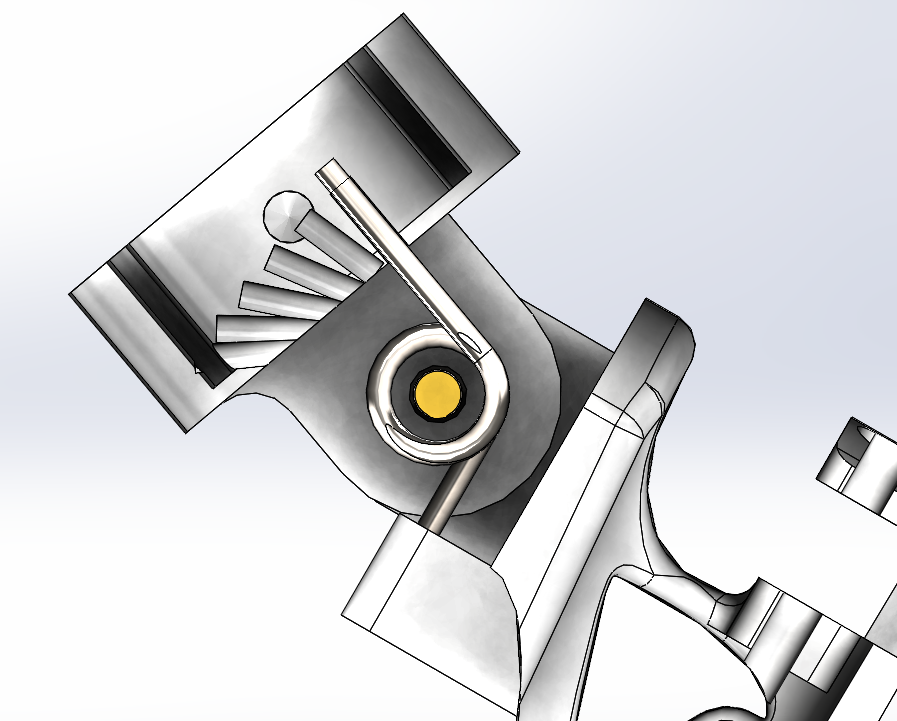
\includegraphics[width=0.75\textwidth]{figures/rotational_spring_rest_positions}
	\caption{Transversal section of the parallel spring resting positions in the left ankle.}
	\label{fig:rotational_spring_rest_position}
\end{figure}

\subsubsection{SEA + PEA configuration} % (fold)
\label{ssub:sea_pea_configuration}
The possibility of using both, SEA and PEA, configurations at the same time is given.
This lets the study of the combination of both configuration.
% subsubsection sea_pea_configuration (end)

\subsubsection{DD configuration } % (fold)
\label{ssub:dd_configuration}
Finally if no parallel spring is used and a spring stiff enough that doesn't add compliance to the system is placed, a DD configuration is achieved.
% subsubsection dd_configuration (end)

% subsection spring_integration (end)